
% this file is called up by thesis.tex
% content in this file will be fed into the main document
% ----------------------- paths to graphics ------------------------

% change according to folder and file names
\ifpdf
    \graphicspath{{8/figures/PNG/}{8/figures/PDF/}{8/figures/}}
\else
    \graphicspath{{8/figures/EPS/}{8/figures/}}
\fi


\chapter{Appendices} % top level followed by section, subsection
\section{Accommodating Single- and Double-regulated hydraulic turbines.}

In order to increase the hydraulic turbine flexibility, in terms of variation in flowrate (Q) and hydraulic head (H), the concept of regulation is used. A regulated hydraulic turbine is a turbine with adjustable blades, either stator or rotor or both. An adjustable blade is a blade that can be rotated around a predefined axis through a specially design mechanism. 


\subsection{Single-regulated turbines}
\label{single.regulated}

Hydraulic turbines that have only one set of adjustable blades (usually they are the stator blades) are called single-regulated turbines (see figure \ref{signle}). Typical examples of this type are; Francis turbines, axial fixed blade propeller turbine has adjustable stator blades and the so called semi-Kaplan concept were fixed stator blades and adjustable rotor blades are used.  
Although the angle of rotation of the adjustable blades ($\alpha$) for each operating point can be treated as additional design variables equal in number to the number of operating points, a different approach is proposed in this thesis. 
                 

\begin{figure}[h!]
\centering
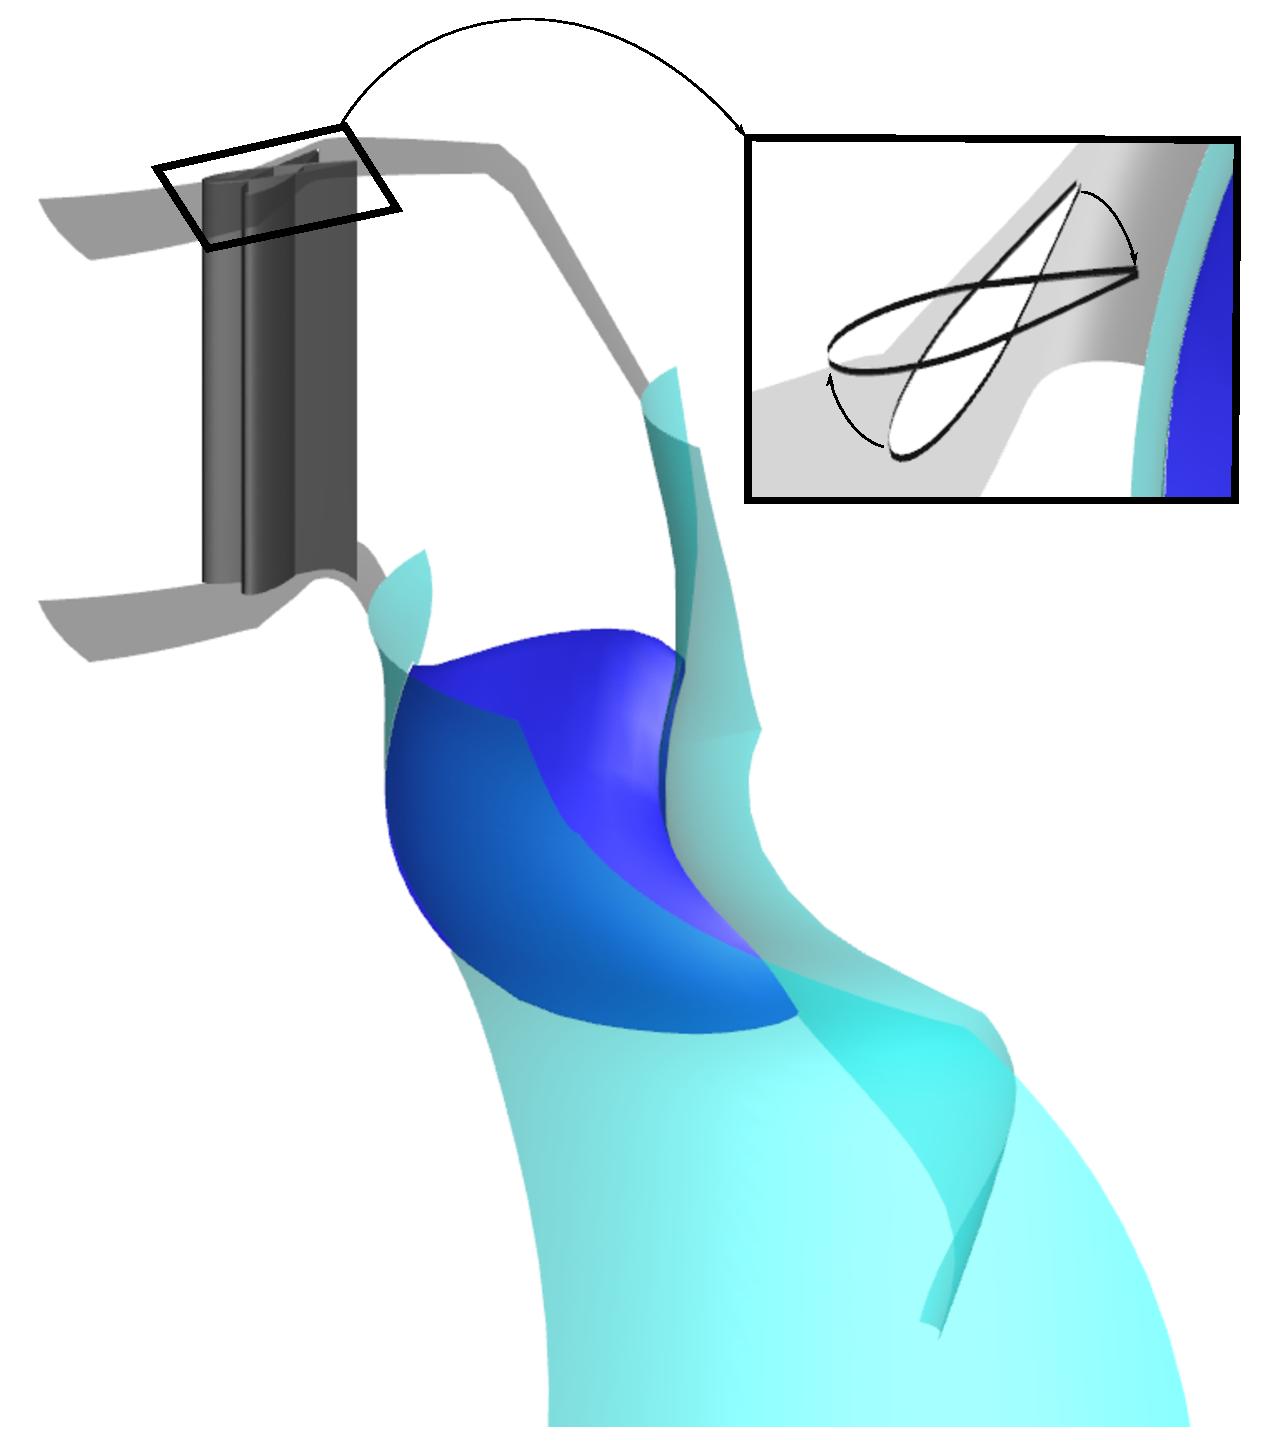
\includegraphics[width=.8\textwidth]{SINGLE.eps}
\caption{Single-regulated turbine.}
\label{signle}
\end{figure}


The proposed approach to the single-regulated turbine problem aims in eliminating both the introduction of the additional constraints and, more importantly, the necessity of imposing the so-called operating point constraints. This is achieved by assuring that each candidate solution will operate at the appropriate $\alpha$ so as to operate at the desirable operating point. Should this be the case, then the quality metrics are computed and the evolution continuous as presented before. 

The aforementioned approach, takes place by enxancing the candidate solution evaluation procedure so at to calculate the appropriate $\alpha$ given the desirable operating point. This is achieved through the algorithm presented below. 
\newpage
For each candidate solution:
\begin{itemize}
\item[]{\bf Step 1:}  (Initialization) 
\begin{itemize}
	\item[]{\bf Step 1a:} (Initial $\alpha$) Set the iteration counted to $i=0$ and $\alpha_i=\alpha _0$ where $\alpha _0$ a user defined value.
	\item[]{\bf Step 1b:} (First step) Set $i=1$ and $\Delta \alpha= \Delta \alpha_0$ where $\Delta \alpha_0$ the user defined magnitude of the first step. Perform the first step:
\begin{eqnarray}
	\alpha_1={\left\{ 
	\begin{array}{ll}
    \alpha_0 - \Delta \alpha_0 ~~,\mbox{if $(Q < Q_{required})$ or ($H > H_{required})$}\\
	\alpha_0 + \Delta \alpha_0 ~~,\mbox{if $(Q > Q_{required})$ or $(H < H_{required})$}\\
    \end{array} \right. }
    \label{step0}
\end{eqnarray}  
It is reminded that $\alpha=0^o$ is the fully open stator position.
\end{itemize}

\item[]{\bf Step 2:}  (Gradient computation) Set $i=i+1$. Compute the gradient of either $\frac{\partial(Q-Q{required})}{\partial \alpha}$ or $\frac{\partial(H-H{required})}{\partial \alpha}$, depending on the chosen boundary conditions of the solver in hand. The two variations are identical. Herein the Q example will be used for space economy. 
\begin{eqnarray}
	\frac{\partial(Q-Q_{required})}{\partial \alpha}=\frac{(Q_{i-1}-Q_{required})-(Q_{i-2}-Q_{required})}{\alpha_{i-1}- \alpha_{i-2}}
\end{eqnarray}  

\item[]{\bf Step 3:}  (Update $\alpha$) Based on the Newton-Raphson method the updated $\alpha$ can be calculated as follows
\begin{eqnarray}
	\alpha_{i}=\alpha_{i-1} - \eta \frac{Q_{i-1}-Q_{required}} {\frac{\partial(Q-Q_{required})}{\partial \alpha}}  
\end{eqnarray}  
where $\eta$ a user defined relaxation factor. 

\item[]{\bf Step 3:} (Finalization check) If $|Q_{i}-Q_{required}|<\Delta Q^*$ end else go to step 2. Where $\Delta Q^*$ a user defined value.
\end{itemize}  

This of course can be scaled, during a multi operating point design problem, to any number of operating points.     

\subsection{Double-regulated turbines}

Hydraulic turbines that have two sets of adjustable blades (rotor and stator) are called double-regulated turbines (see figure \ref{double}). Typical examples of this is the Kaplan turbine.  
Herein the angle of rotation of the adjustable stator blades is denoted as $\alpha$ (in accordance with the previous section) and of the rotor blades as $\beta$. Furthermore, apart from the operation in the desirable operating point, the $C_u$ velocity component at the outlet of the runner at the hub position is required to have the user-defined (through the target $C_u$ distribution) value, the second requirement is denoted as $S$.     
Regarding the operating point requirement, the Q variation will be used as before, having in mind that it could easily be transformed to the H one.  

\begin{figure}[h!]
\centering
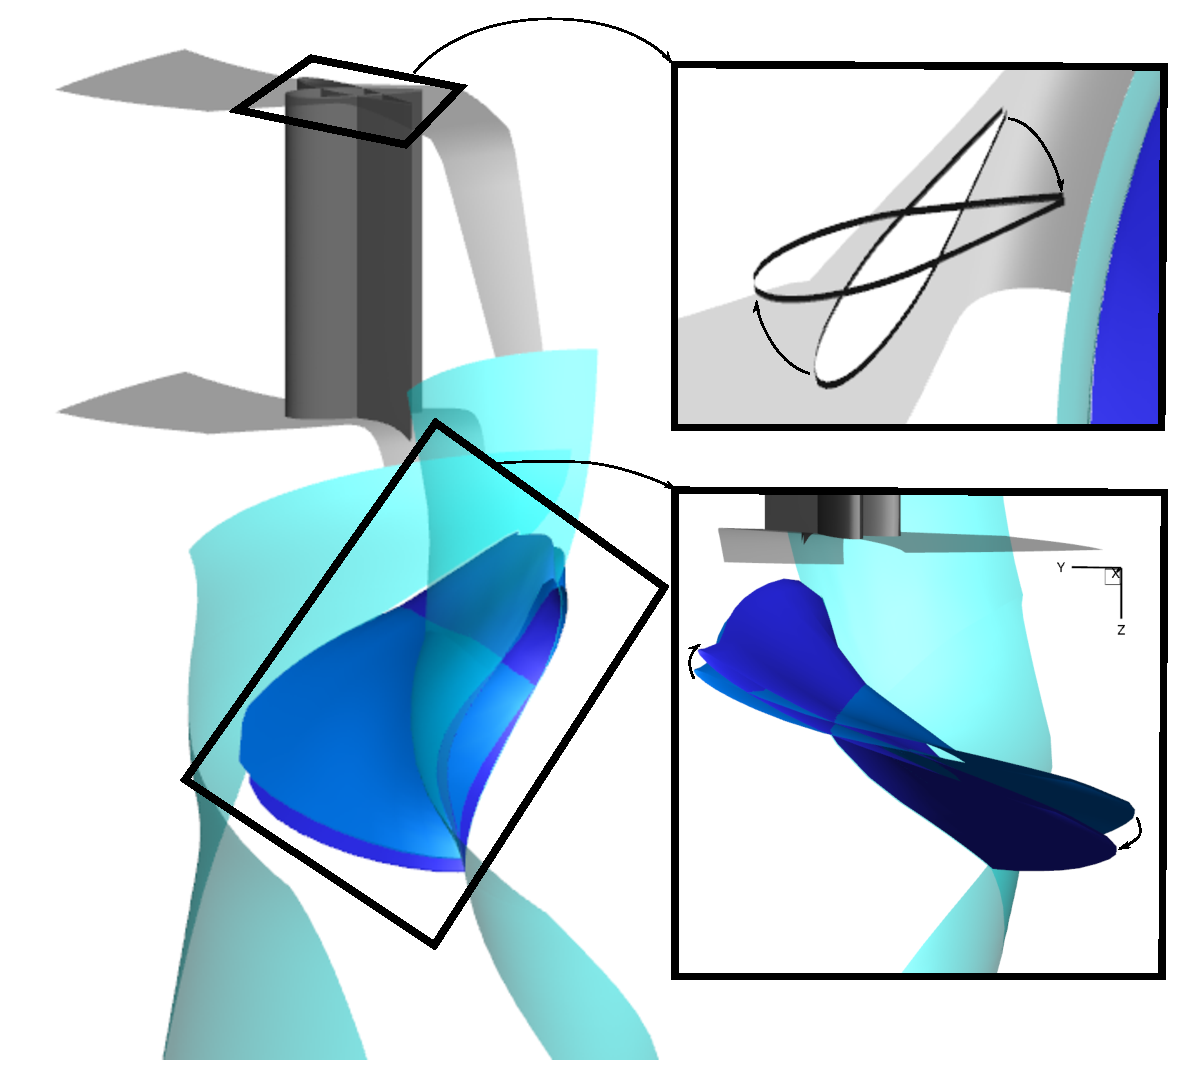
\includegraphics[width=.8\textwidth]{DOUBLE.eps}
\caption{Double-regulated turbine.}
\label{double}
\end{figure}


The algorithm of the approach suitable for double-regulated turbines follows.
For each candidate solution:
\begin{itemize}
\item[]{\bf Step 1:}  (Initialization) 
\begin{itemize}
	\item[]{\bf Step 1a:} (Initial $\alpha$ and $\beta$) Set the iteration counted to $i=0$, $\alpha_i=\alpha _0$ and $\beta_i=\beta _0$ where $\alpha _0$ and $\beta _0$ are user defined value.
	\item[]{\bf Step 1b:} (First step) Set $i=1$, $\Delta \alpha= \Delta \alpha_0$ and $\Delta \beta= \Delta \beta_0$ where $\Delta \alpha_0$ and $\Delta \beta_0$ the user defined magnitude of the first step. Perform the first step:

\begin{eqnarray}
	\alpha_1={\left\{ 
	\begin{array}{ll}
    \alpha_0 - \Delta \alpha_0 ~~,\mbox{if $(Q < Q_{required})$}\\
	\alpha_0 + \Delta \alpha_0 ~~,\mbox{if $(Q > Q_{required})$}\\
    \end{array} \right. }
    \label{step0}
\end{eqnarray}  
It is reminded that $\alpha=0^o$ is the fully open stator position.

and 

\begin{eqnarray}
	\beta_1={\left\{ 
	\begin{array}{ll}
    \beta_0 - \Delta \beta_0 ~~,\mbox{if $(S > 0)$}\\
	\beta_0 + \Delta \beta_0 ~~,\mbox{if $(S < 0)$}\\
    \end{array} \right. }
    \label{step0}
\end{eqnarray}  
It is reminded that $\beta=0^o$ is the fully open rotor position.


\end{itemize}

\item[]{\bf Step 2:}  (Gradient computation) Set $i=i+1$. 
\begin{eqnarray}
	\frac{\partial(Q-Q_{required})}{\partial \alpha}=\frac{(Q_{i-1}-Q_{required})-(Q_{i-2}-Q_{required})}{\alpha_{i-1}- \alpha_{i-2}}
\end{eqnarray}  

\begin{eqnarray}
	\frac{\partial(Q-Q_{required})}{\partial \beta}=\frac{(Q_{i-1}-Q_{required})-(Q_{i-2}-Q_{required})}{\beta_{i-1}- \beta_{i-2}}
\end{eqnarray}  

\begin{eqnarray}
	\frac{\partial(S)}{\partial \alpha}=\frac{S_{i-1}-S_{i-2}}{\alpha_{i-1}- \alpha_{i-2}}
\end{eqnarray}  

\begin{eqnarray}
	\frac{\partial(S)}{\partial \beta}=\frac{S_{i-1}-S_{i-2}}{\beta_{i-1}- \beta_{i-2}}
\end{eqnarray}  

\item[]{\bf Step 3:}  (Update $\alpha$ and $\beta$) Update $\alpha$ and $\beta$ based on the previously computer Gradient.
Similarly to the single-regulated algorithm, the Newton-Raphson method is used.
  
From,  
\begin{eqnarray}
		\left( {\begin{array}{c}
 		\frac{\partial(Q-Q_{required})}{\partial \alpha} \\
 		\frac{\partial(S)}{\partial \alpha}	\\
 		\end{array} } 
 	   {\begin{array}{c}
 		\frac{\partial(Q-Q_{required})}{\partial \beta}  \\
 		\frac{\partial(S)}{\partial \beta}
 		\end{array} } \right)
 		\left( {\begin{array}{c}
 		\Delta \alpha  \\
 		\Delta \beta	\\
 		\end{array} } \right) =
		\left( {\begin{array}{c}
 		Q_{i-1}-Q_{required}  \\
 		S_{i-1}  \\
 		\end{array} } \right)
   \label{cdf-matrix} 
\end{eqnarray}
the $\Delta \alpha$ and $\Delta \beta$ quantities can be, easily computed via a simple $2 \times 2$ matrix inversion.

Finally  $\alpha_i$ and $\beta_i$ are computed by,

\begin{eqnarray}
\alpha_{i}=\alpha_{i-1} - \eta_1 \Delta \alpha  
\end{eqnarray}  
and 
\begin{eqnarray}
\beta_{i}=\beta_{i-1} - \eta_2 \Delta \beta  
\end{eqnarray}  

%\begin{eqnarray}
%\alpha_{i}=\alpha_{i-1} - \eta_1 \frac{Q_{i-1}-Q_{required}} %{\frac{\partial|Q-Q_{required}|}{\partial \alpha}} - \eta_2 %\frac{S_{i-1}}{\frac{\partial(S)}{\partial \alpha}}  
%\end{eqnarray}  
%\begin{eqnarray}
%\beta_{i}=\beta_{i-1} - \eta_1 \frac{Q_{i-1}-Q_{required}} %{\frac{\partial|Q-Q_{required}|}{\partial \beta}} - \eta_2 %\frac{S_{i-1}}{\frac{\partial(S)}{\partial \beta}}  
%\end{eqnarray}  

where $\eta_1$ and $\eta_2$ a user defined relaxation factor. 

\item[]{\bf Step 3:} (Finalization check) If ($|Q_{i}-Q{required}|<\Delta Q^*$) ($AND$ $|S|<S^*$) end else go to step 2. Where $\Delta Q^*$ and $S^*$ are user defined values.
\end{itemize}



\FloatBarrier
\newpage
\section{Experimental Validation of the design of a Hydromatrix$\circledR$}

The experimental validation of a design that took place using the methods presented in this thesis is presented in this section. This design took place in the scope of the EU funded project named ``HYDROACTION – Development and laboratory testing of improved action and Matrix hydro turbines designed by advanced analysis and optimization tool'' (FP7: Project Number 211983). 


The design variable is based on the parameterization (as presented in chapter 5) and is using $52$ design variables to describe the rotor blades mean surface, thickness distribution and hub generatrices (table. \ref{design_vars2}). 


To ensure performance stability, the runner was desired to perform optimally at three operating points (BE, PL and FL), table \ref{epxer.ops}.

\begin{table}[h!]
\begin{center}
\begin{tabular}{ |c|c|c| }
\hline
Operating point & $N_{ED}$ & $Q_{ED}$\\
\hline
BE & $0.97$ & $0.62$\\
\hline
PL       & $1.42$ & $0.84$\\
\hline
FL       & $0.92$ & $0.6$\\
\hline
\end{tabular}
\caption{Experimental Validation of the design of a Hydromatrix$\circledR$: Operating points.}
\label{epxer.ops}
\end{center}
\end{table}

The objectives vector consist of three objectives, first among them ($F_1$) is the outlet velocity profile metric ($M_1$), second ($F_2$) is the combination of (a) blade loading quality metric ($M_2$), (b) the cavitation index $\sigma_{histogram}$, and third ($F_3$) is the pumping surface metric ($M_3$). 

Due to the multi operating point design problem,  three objective $(f_1^{i},f_2^{i},f_3^{i})$ for each operating point $i$ is defined,

\begin{eqnarray}
f_1^i= \alpha ^i M_1^i ~~~\& ~~~ f_2^i =\beta ^i M_2^i +\gamma ^i \sigma_i^{Hist} ~~~\&~~~ f_3^i = \delta ^i M3^i
%   f_1^i= \alpha ^i  M_1^i ~~~\& ~~~ f_2^i=\beta ^i Μ_2^i-\gamma ^i  \sigma^i + \delta ^i  Μ_3^i 
   \label{exp.ObjM} 
\end{eqnarray}

\begin{table}[h!]
\begin{center}
\begin{tabular}{ |l|r|r|r|c| }
%\hline
%\multicolumn{4}{|c|}{Βάρη} & F \\
\hline
& BE, $i\!=\!1$ & PL, $i\!=\!2$ & FL, $i\!=\!3$ &  Associated objective\\
\hline
\greek{α ($M_1$)} & 1.0            &1.0            &1.0 & $f_1$\\
\hline
\greek{β ($M_2$)} &0.2    &0.2            &0.2  & $f_2$\\
\hline
\greek{γ ($\sigma_i^{Hist}$)} &1.0            &1.0            &1.0 & $f_3$\\
\hline
\greek{δ} ($M_3$) &0.0            &100.0  &100.0 & $f_2$\\
\hline
\end{tabular}
\caption{Experimental Validation of the design of a Hydromatrix$\circledR$: Weights associated with the quality-metrics grouping into objectives.}
\label{exp-weights-M1}
\end{center}
\end{table}

Given the already defined $3\!\times\!3\!=\!9$ functions to be minimized at the three operating points, the three objective functions finally used are defined by concatenating the previous ones with weight factors $w_i$, as follows

\begin{equation} 
f_1=\sum^3_{i=1}w_if_1^i ~~~\&~~~ f_2=\sum^3_{i=1}w_if_2^i  ~~~\&~~~ f_3=\sum^3_{i=1}w_if_3^i
\label{exp.F12}
\end{equation}


\begin{table}[h!]
\begin{center}
\begin{tabular}{ |c|l| }
\hline
Operating point & weight, $w_i$\\
\hline
Best efficiency (BE), $i\!=\!1$  & 1.0\\
\hline
Part load  (PL), $i\!=\!2$ & 0.1\\
\hline
Full load (FL), $i\!=\!3$  & 0.1\\
\hline
\end{tabular}
\caption{Experimental Validation of the design of a Hydromatrix$\circledR$: Operating point weights.}
\label{exp.weights}
\end{center}
\end{table}

The resulting front of non-dominated solutions computed at the cost of $2000$ evaluations is presented in figure \ref{exp.pareto}. The upgrade of $\sigma$ from a constrained to an objective gave the ability, with a single optimization run, to acquire a number of designs each of them optimum for different levels of $\sigma$. It is reminded that a design can operate with higher $\sigma$ without suffering from cavitation if its placed deeper, thus having a greater mass of water above it. Also the Hydromatrix$\circledR$ turbines are usually placed on a number of rows one above the other, therefore the aforementioned upgrade of $\sigma$ to an objective gives the ability with only a single run to acquire all turbines needed for an entire project. 

\begin{figure}[h!]
\begin{minipage}[b]{0.5\linewidth}
 \centering
 \resizebox*{8.0cm}{!}{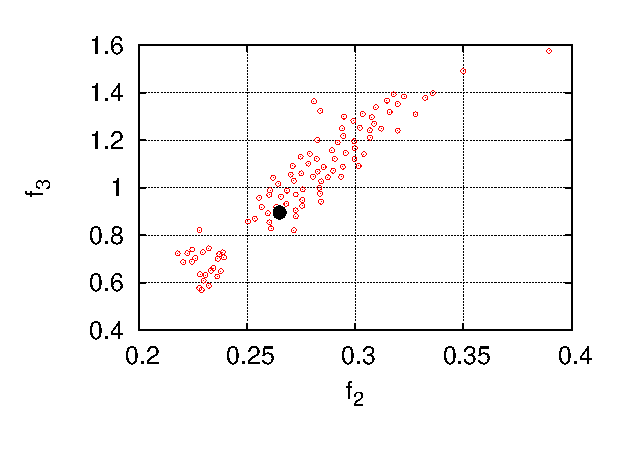
\includegraphics{./3obj6/final_pareto2d2.eps}}
\end{minipage}
\begin{minipage}[b]{0.5\linewidth}
 \centering
 \resizebox*{8.0cm}{!}{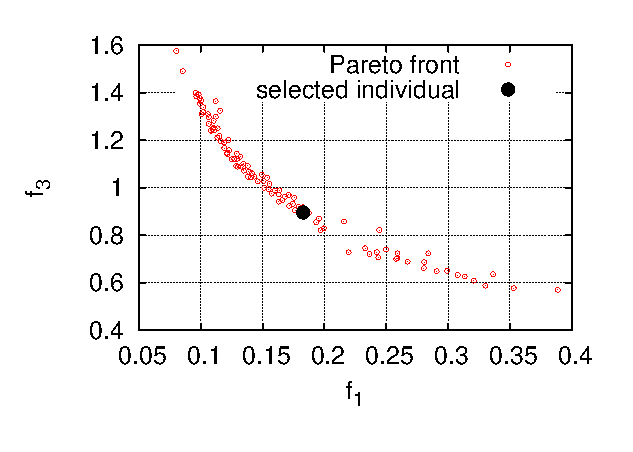
\includegraphics{./3obj6/final_pareto2d3.eps}}
\end{minipage}
\begin{minipage}[b]{0.5\linewidth}
 \centering
 \resizebox*{8.0cm}{!}{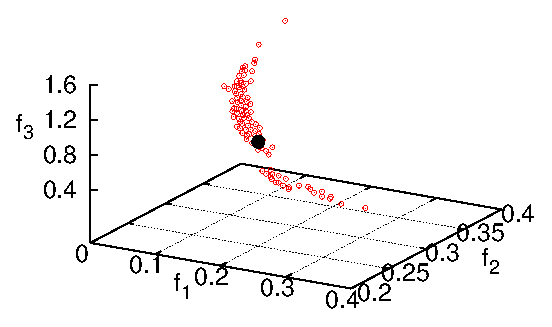
\includegraphics{./3obj6/final_pareto.eps}}
\end{minipage}
\begin{minipage}[b]{0.5\linewidth}
 \centering
 \resizebox*{8.0cm}{!}{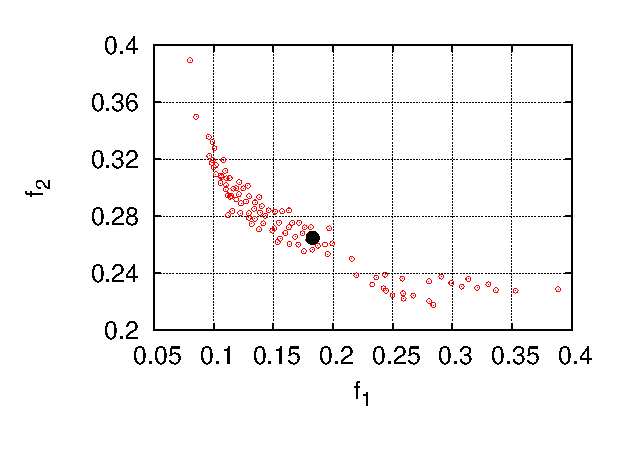
\includegraphics{./3obj6/final_pareto2d1.eps}}
\end{minipage}
\caption{Experimental Validation of the design of a Hydromatrix$\circledR$: The 3D front of non-dominated solutions acquired at the cost of 2000 evaluations. The 3D plot and its projections at the ($[f_2,f_3]$, $[f_1,f_3]$ and $[f_1,f_2]$) are given. This front, resulting from a three objective optimization procedure, allows the designer a variety of choices between optimum designs. This is of grate usefulness especially when dealing with Hydromatrix$\circledR$ turbines since the designer can make different choices for the different rows of the  Hydromatrix$\circledR$ power plant. }
\label{exp.pareto}
\end{figure}

Regarding the experimental validation of the acquired by the proposed in this thesis methods, a single design from the computed front of non-dominated solutions was selected, build and measured           in test rig L2b of Andritz Hydro GmbH in Linz, Austria (see figure \ref{exp.lab}). The selected design will later be compared, efficiency wise, with a reference Hydromatrix$\circledR$ turbine designed to operate at similar operating region.    

Before moving to the experimental results an analysis of the numerical simulations performed for the selected design follows. In figure \ref{exp.BE}-left the high loading quality of the selected design is demonstrated through the $C_p$ chordwise (eq. \ref{Cpdef}) distribution along the hub, mid-span and shroud positions. In figure \ref{exp.BE}-right the excellent agreement of the outlet velocity profiles ($C_m$ and $C_u$) with the desired ones is presented. Furthermore in figure \ref{exp.PL.FL} the $C_p$ distributions demonstrate the loading quality of the selected design when it operates at FL and PL operating point according to their $f_3$ value.    

%\begin{figure}[h!]
%\begin{minipage}[b]{1\linewidth}
% \centering
% \resizebox*{15.0cm}{!}{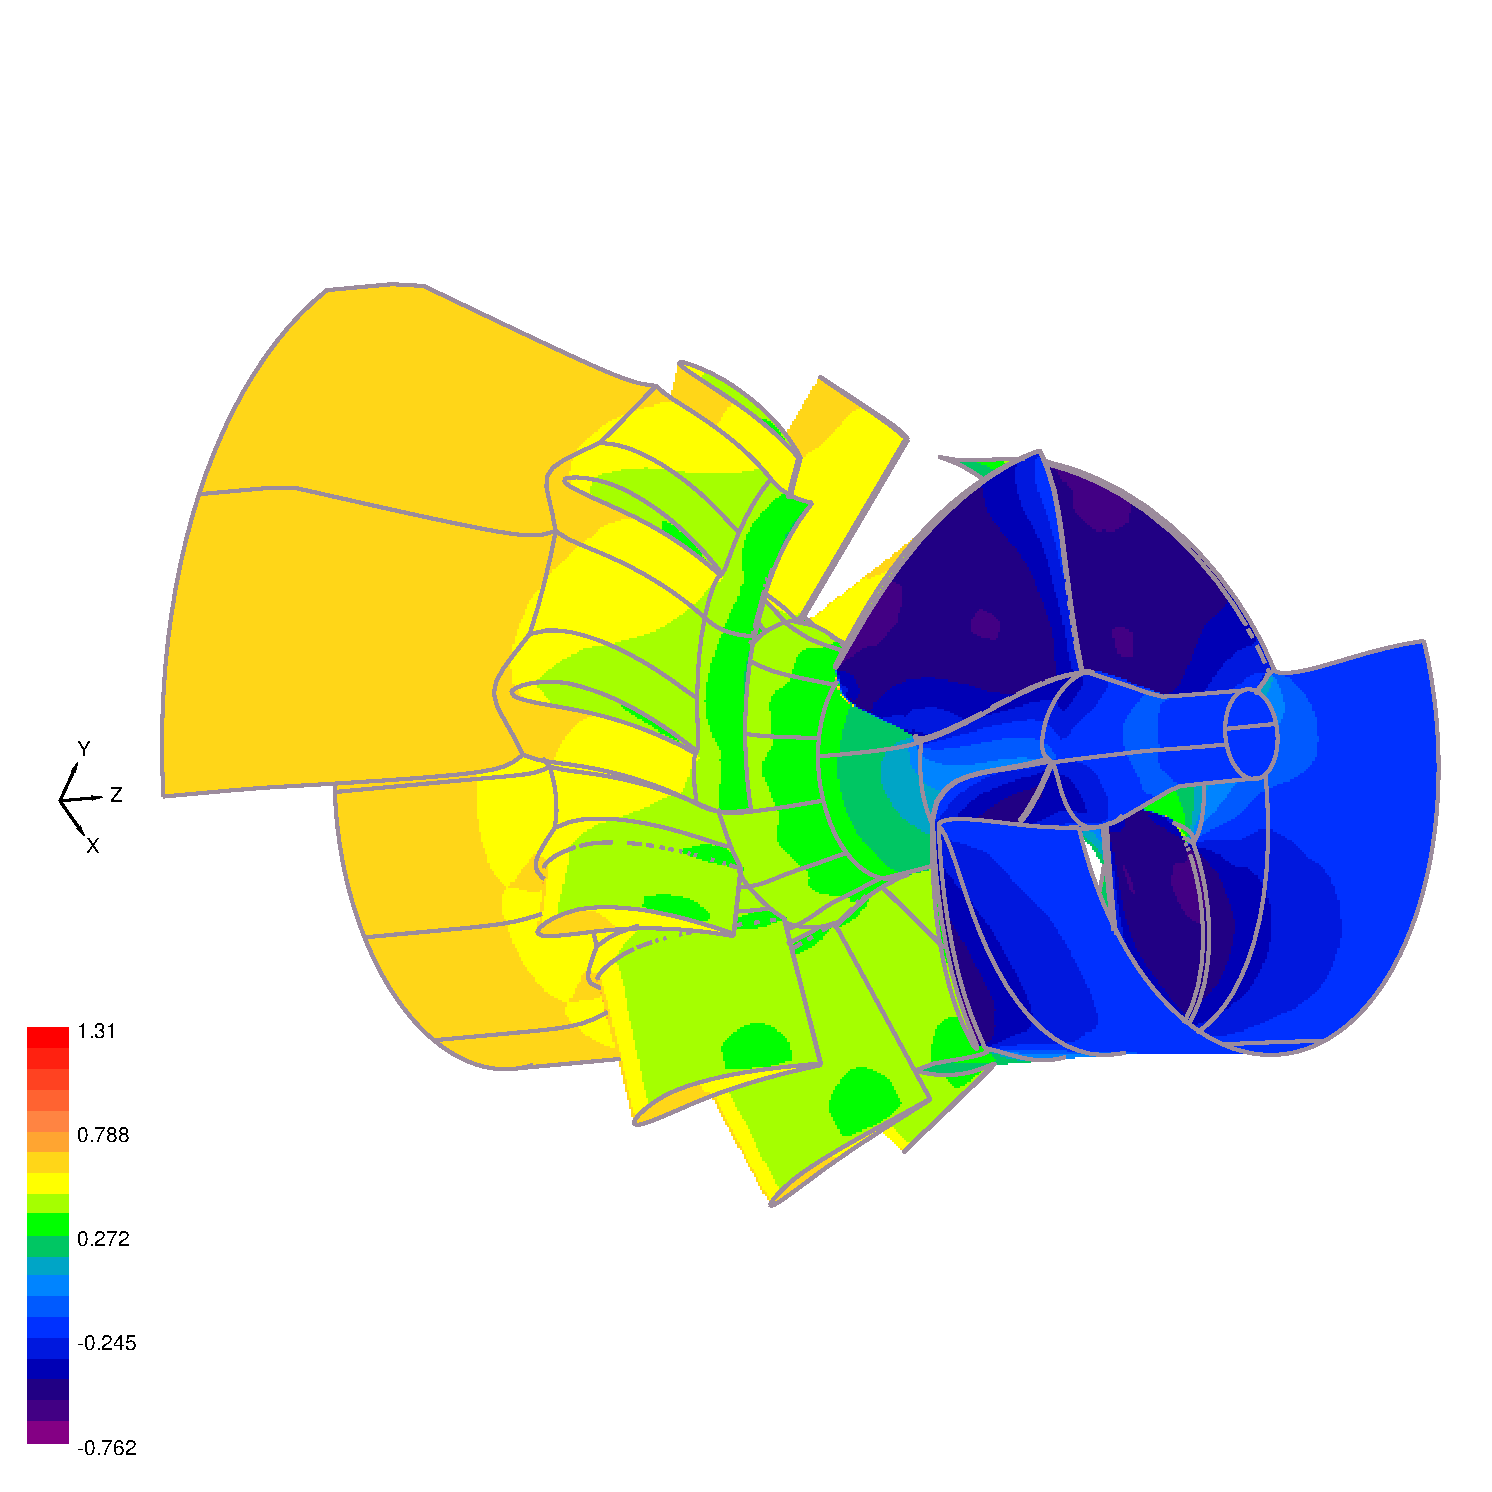
\includegraphics{./3obj6/OP1/AllPress.eps}}
%\end{minipage}
%\caption{Experimental Validation of the design of a Hydromatrix$\circledR$: $\sigma$ contour for design A at BE operating point.}
%\label{exp.All_press.BE}
%\end{figure}


\begin{figure}[h!]
\begin{minipage}[b]{0.5\linewidth}
 \centering
 \resizebox*{7.5cm}{!}{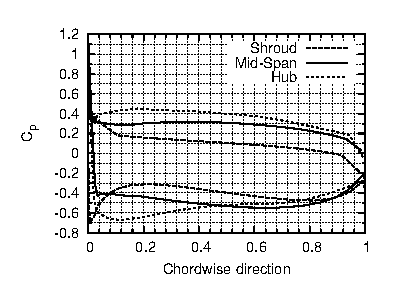
\includegraphics{./3obj6/OP1/LOAD.eps}}
\end{minipage}
\begin{minipage}[b]{0.5\linewidth}
 \centering
 \resizebox*{6.7cm}{!}{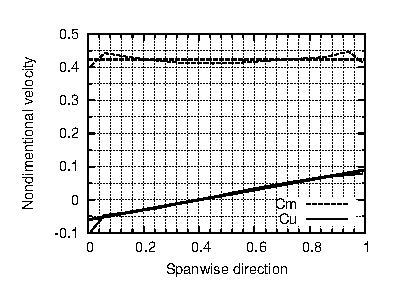
\includegraphics{./3obj6/OP1/OUTLET.eps}}
\end{minipage}

\caption{Experimental Validation of the design of a Hydromatrix$\circledR$: Left: $C_p$ profiles at hub, mid-span and shroud positions for the selected design when it operates at the BE operating point. Right: $C_m$ and $C_u$ outlet velocity profiles forthe selected design at BE operating point}
\label{exp.BE}
\end{figure}
 
 

\begin{figure}[h!]
\begin{minipage}[b]{0.5\linewidth}
 \centering
 \resizebox*{7.5cm}{!}{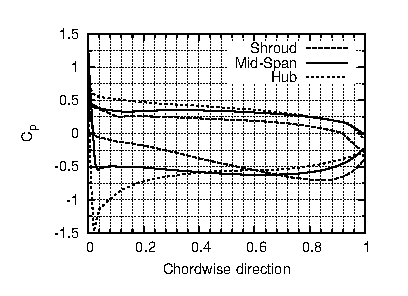
\includegraphics{./3obj6/OP2/LOAD.eps}}
\end{minipage}
\begin{minipage}[b]{0.5\linewidth}
 \centering
 \resizebox*{7.5cm}{!}{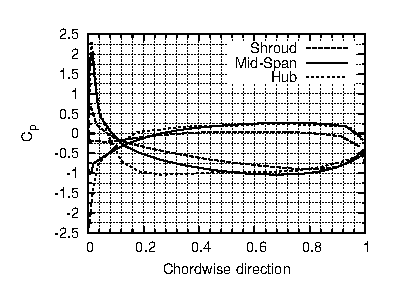
\includegraphics{./3obj6/OP3/LOAD.eps}}
\end{minipage}

\caption{Experimental Validation of the design of a Hydromatrix$\circledR$:  Left: $C_p$ profiles at hub, mid-span and shroud positions for the selected design when it operates at the FL operating point.  Right: $C_p$ profiles at hub, mid-span and shroud positions for the selected design when it operates at the PL operating point}
\label{exp.PL.FL}
\end{figure}

\FloatBarrier
\subsection{Experimental measurement}  
The experimental validation of the Hydromatrix$\circledR$ quality of the selected design was performed on test rig number L2b of Andritz Hydro GmbH in Linz, Austria (see figure \ref{exp.lab}), which is specialized for Bulf, Straflo and Hydromatrix$\circledR$ turbines. In L2b, three pumps are used to create the desirable hydraulic energy (Q,H).  The model turbine is installed between head and tail water tank.

The model head is regulated by the pump speed and the tail
water elevation is simulated by the pressure in the downstream tank. The downstream tank is connected to a vacuum vessel and to compressed air as well. This allows varying the pressure in the downstream tank for the simulation of the necessary cavitation conditions, while keeping the model head constant. For Hydromatrix$\circledR$ tests a special inlet box the simulated the river flow is required.

\begin{figure}[h!]
\centering
\resizebox*{15.0cm}{!}
{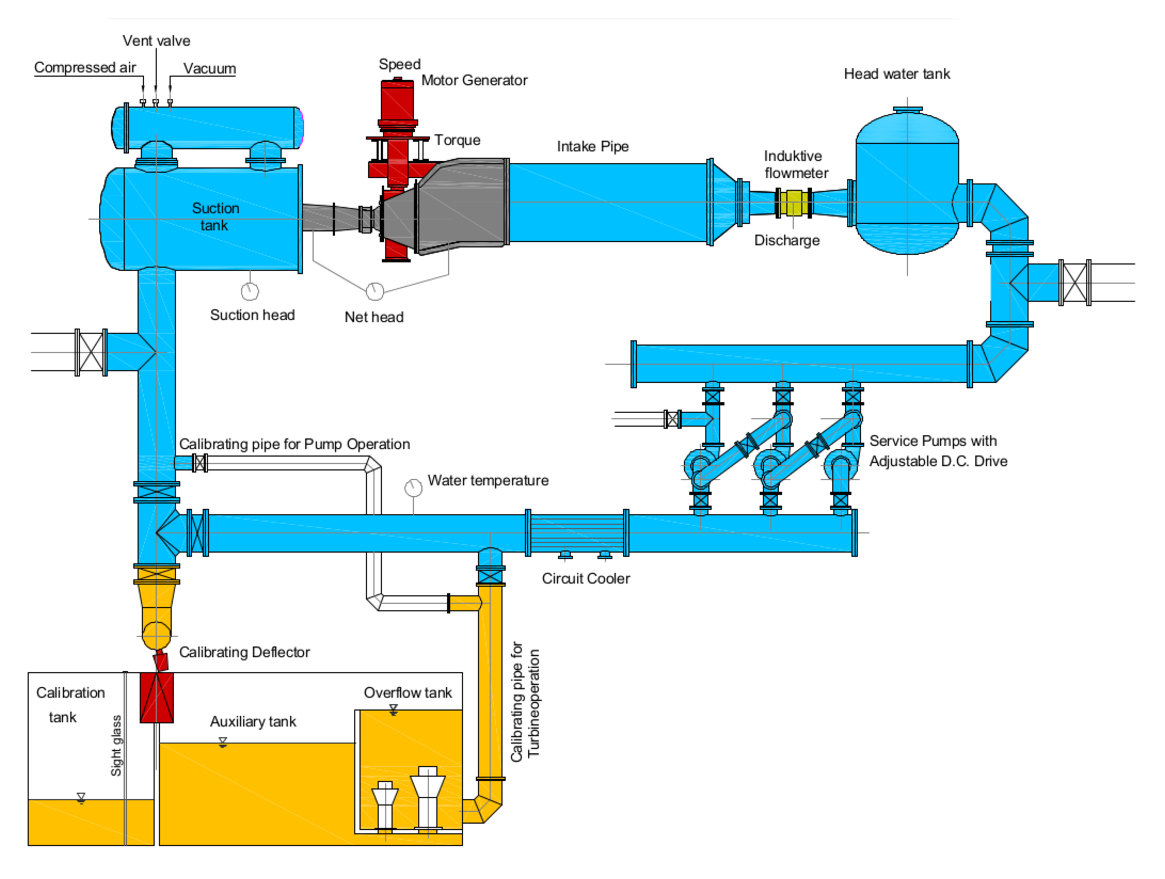
\includegraphics[width=1\textwidth]{lab.eps}}
\caption{Experimental Validation of the design of a Hydromatrix$\circledR$: General layout of test rig L2b in Hydromatrix$\circledR$ turbine configuration.
L2b is operated as a closed loop and is able to perform a variety of tests as indicated in IEC60193.}
\label{exp.lab}
\end{figure}

Regarding the torque measurement a strain-gage equipped shaft whose signal is transported over a wireless telemetry system that forwards the data to the data acquisition system is used. The model head (H) is measured from the static pressure difference between headwater tank and tail water tank and the velocity difference in the measurement sections (distributor cone inlet and draft tube outlet). The massflow (Q) is measured with an inductive discharge flow meter and the rotational speed is measured via a incremental encoder with a resolution of 1024 Impules per revolution. All measuring instruments were calibrated either by primary normals or by using calibration devices which are calibrated with a primary normal. Furthermore the runner blades geometry were checked with a 3D coordinate measurement machine by an external company.

\begin{figure}[h!]
\centering
\resizebox*{13.0cm}{!}
{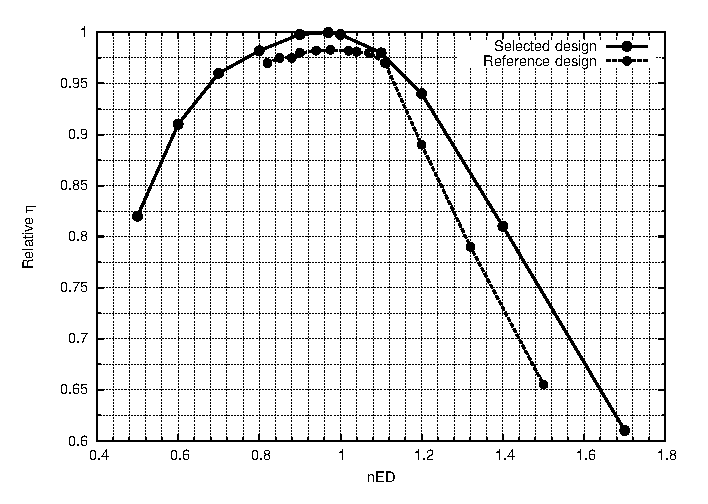
\includegraphics[width=1\textwidth]{./3obj6/Eff.eps}}
\caption{Experimental Validation of the design of a Hydromatrix$\circledR$: Relative efficiency ($\frac{\eta}{max(\eta)}$) charts regarding the reference and selected designs. The selected design, as it was generated using the proposed in this thesis methods, outperforms the reference one on all the operating spectrum.}
\label{exp.eff}
\end{figure}


The efficiency ($\eta$) measurements were performed with at the minimum model Reynolds number of $4 × 10^6$ and minimum specific hydraulic energy of $30J/kg$ as indicated in IEC 60193.
In order to acquire the efficiency curve head and the speed will be changed so as to vary the speed factor nED.  The measured efficiency of the selected design is shown, in comparison with a reference design also measured in the same configuration, in a relative efficiency chart in figure \ref{exp.eff}.    

The experimental validation of a Hydromatrix$\circledR$ design showed that the proposed by this thesis methods can deliver high quality designs, acceptable by industrial standards. Furthermore the overall design time was reduced from approximately $120-140$ days to only $50$. This reduction in time, and therefore resources, combined with the ability to treat turbine parts, such the draft tube, as standardised components (merely requiring their coupling properties) resulted in the reduction of each Hydromatrix$\circledR$ unit by, approximately  one third.

This cost reduction makes economically feasible the application of Hydromatrix$\circledR$ turbines in power plants with even lower H (below 5m, as low as 2m)  and relatively small (smaller than $60m^3/s$) discharges. The economic impact of this improvement can be very important as the current estimations for the potential of sites between 2 and 5 meters is approximately $6,000$ GWh
per year in Europe alone\footnote{This figure is given by ``European Commission, Joint Research Centre, Institute for Energy, energy Systems Evaluation Unit,  Petten, 13 of June 2007'' in  ``Report on the Workshop on Hydropower and Ocean Energy – Part II: Hydropower''.}, a market worth potentially more than a billion Euro per year. The environmental impact, assuming that Hydromatrix$\circledR$ turbines will manage to exploit 5\% of that market by the year 2020 and therefore $300$ GWh/year, is calculated using the relevant conversion factors \footnote{HYDI Statistical release on hydropower energy, market \& policy data 2007-2010 with projections to 2020} to enough to power for more than $84,000$ European households and will save the emission $189,000$ tons of $CO_2$ per year.

  

 





 




% ---------------------------------------------------------------------------
%: ----------------------- end of thesis sub-document ------------------------
% ---------------------------------------------------------------------------



 






